% Created 2019-10-16 Wed 14:07
\documentclass[a4paper]{article}
\usepackage[utf8]{inputenc}
\usepackage[T1]{fontenc}
\usepackage{fixltx2e}
\usepackage{graphicx}
\usepackage{longtable}
\usepackage{float}
\usepackage{wrapfig}
\usepackage{rotating}
\usepackage[normalem]{ulem}
\usepackage{amsmath}
\usepackage{textcomp}
\usepackage{marvosym}
\usepackage{wasysym}
\usepackage{amssymb}
\usepackage{hyperref}
\tolerance=1000
\usepackage{tikz}
\usepackage{amsmath}
\usepackage{mathtools,amssymb}
\usepackage{mathrsfs}
\usepackage{pgfplots}
\pgfplotsset{width=16cm,height=6cm, compat=1.8}
\tikzset{  declare function={    normalpdf(\x,\mu,\sigma)= (2*3.1415*\sigma^2)^(-0.5)*exp(-(\x-\mu)^2/(2*\sigma^2)); }}
\author{nybo}
\date{\today}
\title{main}
\hypersetup{
  pdfkeywords={},
  pdfsubject={},
  pdfcreator={Emacs 25.2.2 (Org mode 8.2.10)}}
\begin{document}

\maketitle
\tableofcontents

\newpage
\section{Least squares}
\label{sec-1}

Simple example

\begin{center}
\begin{tabular}{rr}
\# ($n$) & Ohms ($y_n$)\\
\hline
1 & 1068\\
2 & 988\\
3 & 1002\\
4 & 996\\
\end{tabular}
\end{center}

the measurement model and the associated error

$$\begin{array}{ll}
{y_{1}=x+v_{1}} & {e_{1}^{2}=\left(y_{1}-x\right)^{2}} \\
 {y_{2}=x+v_{2}} & {e_{2}^{2}=\left(y_{2}-x\right)^{2}} \\
 {y_{3}=x+v_{3}} & {e_{3}^{2}=\left(y_{3}-x\right)^{2}} \\
 {y_{4}=x+v_{4}} & {e_{4}^{2}=\left(y_{4}-x\right)^{2}}
\end{array}$$

minimizing the error

$$\hat{x}_{\mathrm{LS}}=\operatorname{argmin}_{x}\left(e_{1}^{2}+e_{2}^{2}+e_{3}^{2}+e_{4}^{2}\right)=\mathscr{L}_{\mathrm{LS}}(x)$$

$$\begin{aligned} 
\mathbf{e} &= \left[\begin{array}{l}{e_{1}} \\ {e_{2}} \\ {e_{3}} \\ {e_{4}}\end{array}\right]  =\mathbf{y}-\mathbf{H} x \\
&=\left[\begin{array}{l}{y_{1}} \\ {y_{2}} \\ {y_{3}} \\ {y_{4}}\end{array}\right]-\left[\begin{array}{l}{1} \\ {1} \\ {1} \\ {1}\end{array}\right] x 
\end{aligned}$$

Squared error, what we want to minimize

$$\begin{aligned} 
  \mathscr{L}_{\mathrm{LS}}(x)=e_{1}^{2}+e_{2}^{2}+e_{3}^{2}+e_{4}^{2} 
&=\mathbf{e}^{T} \mathbf{e} \\ &=(\mathbf{y}-\mathbf{H} x)^{T}(\mathbf{y}-\mathbf{H} x) 
\\ &=\mathbf{y}^{T} \mathbf{y}-x^{T} \mathbf{H}^{T} \mathbf{y}-\mathbf{y}^{T} \mathbf{H} x+x^{T} 
\mathbf{H}^{T} \mathbf{H} x 
\end{aligned}$$

To get the smallest sol we do the derivative

$$\begin{aligned}
{ \left.\frac{\partial \mathscr{L}}{\partial x}\right|_{x=\hat{x}}=-\mathbf{y}^{T} \mathbf{H}-\mathbf{y}^{T} \mathbf{H}+2 \hat{x}^{T} \mathbf{H}^{T} \mathbf{H}=0} \\
 {-2 \mathbf{y}^{T} \mathbf{H}+2 \hat{x}^{T} \mathbf{H}^{T} \mathbf{H}=0    }
 \end{aligned}$$


solving
$${\qquad \hat{x}_{\mathrm{LS}}=\left(\mathbf{H}^{T} \mathbf{H}\right)^{-1} \mathbf{H}^{T} \mathbf{y}}$$
X hat minimizes our squared errors. Note: this is only possible if $H$
is not singular / has an inverse. This can be stated as the dimentions
sadifying $n \geq m$, aka more mesurments than states.

$$\mathbf{y}=\left[\begin{array}{c}{1068} \\ {988} \\ {1002} \\ {996}\end{array}\right] \quad \mathbf{H}=\left[\begin{array}{l}{1} \\ {1} \\ {1} \\ {1}\end{array}\right]$$

$$\hat{x}_{\mathrm{LS}}=\left([11111]\left[\begin{array}{l}{1} \\ {1} \\ {1} \\ {1}\end{array}\right]\right)^{-1}[11111]\left[\begin{array}{c}{1068} \\ {988} \\ {1002} \\ {996}\end{array}\right] = 1013.5$$

\newpage

\section{Weigted least squares}
\label{sec-2}

We migt want to weight the mesurments because we might have better
sensores that we trust more.

\begin{center}
\begin{tabular}{rrl}
\# & mulitmeter-A ($\sigma=20$ Ohm) & mulitmeter-B (\$$\sigma$=2\$Ohm)\\
\hline
1 & 1068 & \\
2 & 988 & \\
3 &  & 1002\\
4 &  & 996\\
\end{tabular}
\end{center}

$$\begin{aligned}\left[\begin{array}{l}{y_{1}} \\ {\vdots} \\ {y_{m}}\end{array}\right] &=\mathbf{H}\left[\begin{array}{c}{x_{1}} \\ {\vdots} \\ {x_{n}}\end{array}\right]+\left[\begin{array}{c}{v_{1}} \\ {\vdots} \\ {v_{m}}\end{array}\right] \\ \mathbf{y} &=\mathbf{H x}+\mathbf{v} \end{aligned}$$

Each time varying noiseterm $\mathbf{v_i}$ is an independent random
variable across measurements and has an an different variance ( or
standard deviation) accociated with it.

$$\mathrm{E}\left[v_{i}^{2}\right]=\sigma_{i}^{2}, \quad(i=1, \ldots, m) \quad \mathbf{R}=\mathbb{E}\left[\mathbf{v} \mathbf{v}^{T}\right]=\left[\begin{array}{ccc}{\sigma_{1}^{2}} & {} & {0} \\ {} & {\ddots} & {} \\ {0} & {} & {\sigma_{m}^{2}}\end{array}\right]$$

Each squared error term is now weighted by the inverse of the variance
associated with the corresponding measurement.

$$\begin{aligned} \mathscr{L}_{\mathrm{WLS}}(\mathbf{x}) &=\mathbf{e}^{T} \mathbf{R}^{-1} \mathbf{e} \\ &=\frac{e_{1}^{2}}{\sigma_{1}^{2}}+\frac{e_{2}^{2}}{\sigma_{2}^{2}}+\ldots+\frac{e_{m}^{2}}{\sigma_{m}^{2}} \end{aligned} \quad \text { where } \quad\left[\begin{array}{c}{e_{1}} \\ {\vdots} \\ {e_{m}}\end{array}\right]=\mathbf{e}=\left[\begin{array}{c}{y_{1}} \\ {\vdots} \\ {y_{m}}\end{array}\right]-\mathbf{H}\left[\begin{array}{c}{x_{1}} \\ {\vdots} \\ {x_{n}}\end{array}\right]$$

We approach it's minimization the same way as before,

$$\begin{aligned} \mathscr{L}_{\mathrm{WLS}}(\mathbf{x}) &=\mathbf{e}^{T} \mathbf{R}^{-1} \mathbf{e} \\ &=(\mathbf{y}-\mathbf{H} \mathbf{x})^{T} \mathbf{R}^{-1}(\mathbf{y}-\mathbf{H} \mathbf{x}) \end{aligned}$$

Solving in the same mannor

$$\begin{array}{c}
  \frac{\partial \mathscr{L}}{\partial \mathbf{x}}_{\mathbf{x}=\mathbf{\hat{x}}}
=\mathbf{0}=-\mathbf{y}^{T} \mathbf{R}^{-\mathbf{I}} \mathbf{H}+\hat{\mathbf{x}}^{T} 
\mathbf{H}^{T} \mathbf{R}^{-1} \mathbf{H} 
\end{array}$$

$$\mathbf{H}^{T} \mathbf{R}^{-1} \mathbf{H} \hat{\mathbf{x}}_{\text{WLS}}=\mathbf{H}^{T} \mathbf{R}^{-1} \mathbf{y}$$

we get

$$\hat{\mathbf{x}}=\left(\mathbf{H}^{T} \mathbf{R}^{-1} \mathbf{H}\right)^{-1} \mathbf{H}^{T} \mathbf{R}^{-1} \mathbf{y}$$

An example
$$\mathbf{H}=\left[\begin{array}{l}{1} \\ {1} \\ {1} \\ {1}\end{array}\right] \quad \mathbf{y}=\left[\begin{array}{c}{1068} \\ {988} \\ {1002} \\ {996}\end{array}\right] \quad \mathbf{R}=\left[\begin{array}{cccc}{\sigma_{1}^{2}} & {} & {} & {}  \\ {} &  {\sigma_{2}^{2}} & {}  & {} \\  {} & {} &  {\sigma_{3}^{2}} & {} \\ {} & {} & {} & {\sigma_{4}^{2}}\end{array}\right]=
\left[\begin{array}{cccc}{400} & {}  & {}  & {} \\ 
                         {} & {400}  & {}   & {}  \\ 
                         {} & {} & {4} & {}  \\ 
                         {} & {} & {} & {4}
\end{array}\right]$$

$$\begin{aligned} \hat{x}_{\mathrm{WLS}} &=\left(\mathbf{H}^{T} \mathbf{R}^{-1} \mathbf{H}\right)^{-1} \mathbf{H}^{T} \mathbf{R}^{-1} \mathbf{y} \\ &=\left([1111]\left[\begin{array}{cccc}{400} & {}  & {}  & {} \\ 
                         {} & {400}  & {}   & {}  \\ 
                         {} & {} & {4} & {}  \\ 
                         {} & {} & {} & {4}
\end{array}\right]^{-1}
\left[\begin{array}{l}{1} \\ {1} \\ {1} \\ {1}\end{array}\right]
\right)^{-1}[11111]\left[\begin{array}{cccc}{400} & {}  & {}  & {} \\ 
                         {} & {400}  & {}   & {}  \\ 
                         {} & {} & {4} & {}  \\ 
                         {} & {} & {} & {4}
\end{array}\right]^{-1}\left[\begin{array}{c}{1068} \\ {988} \\ {1002} \\ {996}\end{array}\right] \\
 &= \frac{1}{1 / 400+1 / 400+1 / 4+1 / 4}\left(\frac{1068}{400}+\frac{988}{400}+\frac{1002}{4}+\frac{996}{4}\right) \\
 &= 999.3\end{aligned}$$

Summery

$$\begin{array}{cc}
{\mathscr{L}_{\mathrm{LS}}(\mathbf{x})=\mathbf{e}^{T} \mathbf{e}} & 
{\mathscr{L}_{\mathrm{WLS}}(\mathbf{x})=\mathbf{e}^{T} \mathbf{R}^{-1} \mathbf{e}} \\
 {\hat{\mathbf{x}}_{\mathrm{LS}}=\left(\mathbf{H}^{T} \mathbf{H}\right)^{-1} \mathbf{H}^{T} \mathbf{y}} 
& {\hat{\mathbf{x}}_{\mathrm{WLS}}=\left(\mathbf{H}^{T} \mathbf{R}^{-1} \mathbf{H}\right)^{-1} \mathbf{H}^{T} 
\mathbf{R}^{-1} \mathbf{y}} \\ {m \geq n} & {m \geq n} \\ {} & {\sigma_{i}^{2}>0}
\end{array}$$

\begin{center}
\begin{tabular}{rr}
Current (A) & Voltage (V)\\
\hline
0.2 & 1.23\\
0.3 & 1.38\\
0.4 & 2.06\\
0.5 & 2.47\\
0.6 & 3.17\\
\end{tabular}
\end{center}


\newpage

\section{Recursive Least Squares}
\label{sec-3}

Teqniue that can be used when you dont want to compute the whole badge
at a time.
$$\begin{aligned} \mathscr{L}_{\mathrm{RLS}} &=\mathbb{E}\left[\left(x_{k}-\hat{x}_{k}\right)^{2}\right] \\ &=\sigma_{k}^{2} \end{aligned}$$
Generalizing this to the sates $n$
$$\begin{aligned} \mathscr{L}_{\mathrm{RIS}} &=\mathbb{E}\left[\left(x_{1 k}-\hat{x}_{1 k}\right)^{2}+\ldots+\left(x_{n k}-\hat{x}_{n k}\right)^{2}\right] \\ &=\operatorname{Trace}\left(\mathbf{P}_{k}\right) \end{aligned}$$
$\mathbf{P}_{k}$ is the state covariance matrix. We can forumate a
recursive deeition of this $\mathbf{P}_{k}$ as a funciton of
$\mathbf{K}_{k}$, by using matrix calculus and derivatives
$$\mathbf{P}_{k}=\left(\mathbf{1}-\mathbf{K}_{k} \mathbf{H}_{k}\right) \mathbf{P}_{k-1}\left(\mathbf{1}-\mathbf{K}_{k} \mathbf{H}_{k}\right)^{T}+\mathbf{K}_{k} \mathbf{R}_{k} \mathbf{K}_{k}^{T}$$

$$\mathbf{K}_{k}=\mathbf{P}_{k-1} \mathbf{H}_{k}^{T}\left(\mathbf{H}_{k} \mathbf{P}_{k-1} \mathbf{H}_{k}^{T}+\mathbf{R}_{k}\right)^{-1}$$

$$\begin{aligned} \mathbf{P}_{k} &=\mathbf{P}_{k-1}-\mathbf{K}_{k} \mathbf{H}_{k} \mathbf{P}_{k-1} \\ &=\left(\mathbf{1}-\mathbf{K}_{k} \mathbf{H}_{k}\right) \mathbf{P}_{k-1} \end{aligned}$$

The larger our gain matrix $\mathbf{H}$, the smaller our new estimator
covariance will be. Intuitively, you can think of this gain matrix as
balancing the information we get from our prior estimate and the
information we receive from our new measurement.

\subsubsection{Algorithm}
\label{sec-3-0-1}

\begin{enumerate}
\item We initialize the algorithm with estimate of our unknown parameters
and a corresponding covariance matrix. This initial guess could come
from the first measurement we take and the covariance could come from
technical specifications.
$$\begin{aligned} \hat{\mathbf{x}}_{0} &=\mathbb{E}[\mathbf{x}] \\ \mathbf{P}_{0} &=\mathbb{E}\left[\left(\mathbf{x}-\hat{\mathbf{x}}_{0}\right)\left(\mathbf{x}-\hat{\mathbf{x}}_{0}\right)^{T}\right] \end{aligned}$$

\item Set up our measurement model and pick values for our measurement
covariance.
$$\mathbf{y}_{k}=\mathbf{H}_{k} \mathbf{x}+\mathbf{v}_{k}$$

\item Update the estimate and the covariance:
$$\begin{aligned} \mathbf{K}_{k} &=\mathbf{P}_{k-1} \mathbf{H}_{k}^{T}\left(\mathbf{H}_{k} \mathbf{P}_{k-1} \mathbf{H}_{k}^{T}+\mathbf{R}_{k}\right)^{-1} \\ \hat{\mathbf{x}}_{k} &=\hat{\mathbf{x}}_{k-1}+\mathbf{K}_{k}\left(\mathbf{y}_{k}-\mathbf{H}_{k} \hat{\mathbf{x}}_{k-1}\right) \\ \mathbf{P}_{k} &=\left(\mathbf{1}-\mathbf{K}_{k} \mathbf{H}_{k}\right) \mathbf{P}_{k-1} 
   \end{aligned}$$
\end{enumerate}

\newpage

\section{Least Squares, Method of Maximum Likelihood}
\label{sec-4}

Ganger alle gausian med hverandere
$$\begin{aligned} p(\mathbf{y} | x) & \propto \mathcal{N}\left(y_{1} ; x, \sigma^{2}\right) \mathcal{N}\left(y_{2} ; x, \sigma^{2}\right) \times \ldots \times \mathcal{N}\left(y_{m} ; x, \sigma^{2}\right) \\ &=\frac{1}{\sqrt{(2 \pi)^{m} \sigma^{2 m}}} \exp \left(\frac{-\sum_{i=1}^{m}\left(y_{i}-x\right)^{2}}{2 \sigma^{2}}\right)
\end{aligned}$$ Prøver vi å makisimere

$$\begin{aligned} \hat{x}_{\mathrm{MLE}} &=\underset{x}{\operatorname{argmax}} p(\mathbf{y} | x) \\ &=\underset{x}{\operatorname{argmax}} \log p(\mathbf{y} | x) \end{aligned}$$

Take the log and get something we are farmilliar
$$\log p(\mathbf{y} | x)=-\frac{1}{2 R}\left(\left(y_{1}-x\right)^{2}+\ldots+\left(y_{m}-x\right)^{2}\right)+C$$

$$\hat{x}_{\mathrm{MLE}}=\underset{x}{\operatorname{argmin}} \frac{1}{2 \sigma^{2}}\left(\left(y_{1}-x\right)^{2}+\ldots+\left(y_{m}-x\right)^{2}\right)$$

$$\hat{x}_{\mathrm{MLE}}=\underset{x}{\operatorname{argmin}} \frac{1}{2}\left(\frac{\left(y_{1}-x\right)^{2}}{\sigma_{1}^{2}}+\ldots+\frac{\left(y_{m}-x\right)^{2}}{\sigma_{m}^{2}}\right)$$

$$\hat{x}_{\mathrm{MHE}}=\hat{x}_{\mathrm{LS}}=\underset{x}{\operatorname{argmin}} 
 \mathscr{L}_{\mathrm{LS}}(x)=\underset{x}{\operatorname{argmax}} \mathscr{S}_{\mathrm{MHE}}(x)$$

Good, but sensetive for outliers


\newpage

\newpage

\section{Kalman}
\label{sec-5}
\subsection{Linear dynamical system}
\label{sec-5-1}

\begin{figure}[!h]
\centering
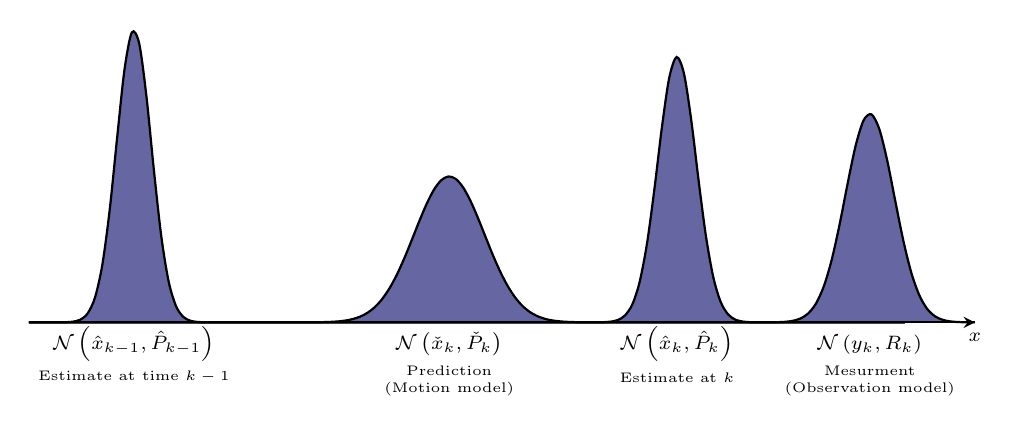
\begin{tikzpicture}[  font=\scriptsize  , >=stealth, Blue/.style={    draw=none, text opacity=1, fill=blue!40!black, fill opacity=0.6  }]
  \begin{axis}[  hide axis,samples=120  , clip= false]
    \addplot[Blue, draw, smooth, thick, domain=0:25]
    {normalpdf(x,3,0.5)};
    \node  at (30,-60) {$\mathcal{N}\left(\hat{x}_{k-1}, \hat{P}_{k-1}\right) $};
    \node[font=\tiny]  at (30,-150) {Estimate at time $k-1$};

    \addplot[Blue, draw, smooth, thick, domain=0:25]
    {normalpdf(x,12,1)};
    \node  at (120,-60) {$ \mathcal{N}\left(\check{x}_{k}, \check{P}_{k}\right) $};
    \node[align=center, font=\tiny]  at (120,-160) { Prediction \\ (Motion model)};

    \addplot[Blue, draw, smooth, thick, domain=0:25] 
    {normalpdf(x,18.5,0.55)} ;
    \node  at (185,-60) {$  \mathcal{N}\left(\hat{x}_{k}, \hat{P}_{k}\right) $};
    \node[font=\tiny]  at (185,-150) {  Estimate at $k$};

    \addplot[Blue, draw, smooth, thick, domain=0:27]
    {normalpdf(x,24,0.7)} ;
    \node  at (240,-60) {$\mathcal{N}\left(y_{k}, R_{k}\right)$};
    \node[align=center, font=\tiny]  at (240,-160) {  Mesurment \\  (Observation model)};

    \draw[->, smooth, thick] (0,0) -- (270,0) node[below] {$x$};
  \end{axis}
  \end{tikzpicture}
\end{figure}

\begin{equation*}
\begin{array}{rlllll}
{\text { Motion model: }} & {\mathbf{x}_{k}=\mathbf{F}_{k-1} \mathbf{x}_{k-1}&+&\mathbf{G}_{k-1} \mathbf{u}_{k-1}&+&\mathbf{w}_{k-1}} \\
{\text { Measurement model: }} & {\mathbf{y}_{k}=\mathbf{H}_{k}   \mathbf{x}_{k}  & &                                 &+&\mathbf{v}_{k}}\vspace{0.4cm} \\ 
 {\text {\ Process or Motion Noise }}& {\mathbf{w}_{k} \sim \mathscr{N}\left(\mathbf{0}, \mathbf{Q}_{k}\right)} &&&\\
 {\text { Measurement Noise }} &{\mathbf{v}_{k} \sim \mathscr{N}\left(\mathbf{0}, \mathbf{R}_{k}\right)}&&& 
\end{array}
\end{equation*}



\vspace{0.6cm}

\begin{equation*}
\begin{array}{rl}
{\check{\mathbf{x}}_{k}} & \text{ { Prediction } \\  { (given motion model) } \\  { at time } k} \\
 {\hat{\mathbf{x}}_{k}} & \text { {Corrected prediction}  \\  { (given measurement) } \\ {\text  at time  k}}
\end{array}
\end{equation*}

\vspace{0.6cm}


\begin{equation*}
\begin{array}{rl}
\text {  Prediction }&
\begin{cases}
{\check{\mathbf{x}}_{k}=\mathbf{F}_{k-1} \mathbf{x}_{k-1}+\mathbf{G}_{k-1} \mathbf{u}_{k-1}} \\ {\hat{\mathbf{P}}_{k}=\mathbf{F}_{k-1} \hat{\mathbf{P}}_{k-1} \mathbf{F}_{k-1}^{T}+\mathbf{Q}_{k-1}}
\end{cases} \vspace{0.6cm} \\
& \qqaud \mathbf{K}_{k}=\check{\mathbf{P}}_{k} \mathbf{H}_{k}^{T}\left(\mathbf{H}_{k} \check{\mathbf{P}}_{k} \mathbf{H}_{k}^{T}+\mathbf{R}_{k}\right)^{-1} \vspace{0.2cm} \\
\text{ \text { Measurement \& Correction }}&
\begin{cases}
{\hat{\mathbf{x}}_{k}=\check{\mathbf{x}}_{k}+\mathbf{K}_{k}\left(\mathbf{y}_{k}-\mathbf{H}_{k} \check{\mathbf{x}}_{k}\right)} \\ {\hat{\mathbf{P}}_{k}=\left(\mathbf{1}-\mathbf{K}_{k} \mathbf{H}_{k}\right) \check{\mathbf{P}}_{k}}
\end{cases}
\end{array}
\end{equation*}
% Emacs 25.2.2 (Org mode 8.2.10)
\end{document}